Die Warenabgabe im Verkauf und der Vermietung erfolgt in einem Ladengeschäft mittels handgeschriebener Rechnungen und Aufträge. Im Anschluss werden die Aufträge und Rechnungen zur weiteren Verwendung in das bestehende MS DOS System wiederholt händisch übertragen. Im darauf folgenden Unternehmensablauf werden die handgeschriebenen Belege an die Buchhaltungsabteilung zur Prüfung des Rechnungseingangs und Rechnungsausgangs sowie an die Fertigungsabteilung zur Auftragsbearbeitung weitergereicht. \cite{einleitung1}
\begin{figure}[!ht]
    \centering
    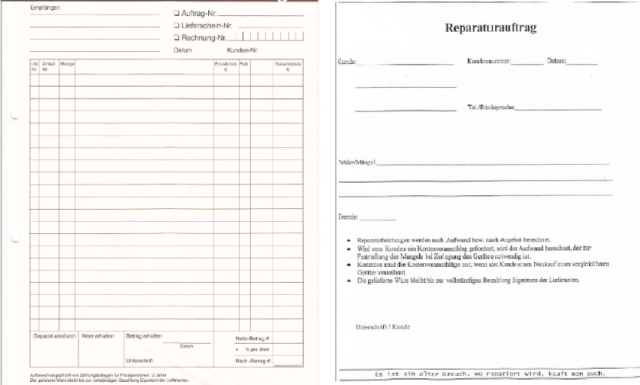
\includegraphics{rechnungReparaturAlt2.png}
    \caption[Muster Rechnungsvordruck und Reparaturauftrag]{\small{Muster eines Rechnungsvordruck (li.) und Reparaturauftrag (re.) \cite{einleitung1}}}
    \label{fig:4}
\end{figure}